\documentclass[11pt]{article}

%FOR SCRIBES: Please change the next three lines to reflect the correct
%FOR SCRIBES: lecture number, name, and date.
\newcommand{\lecturenumber}{4}
\newcommand{\scribename}{Abdullah AlJasser, Andrew McBurnett, Robert Terpin}
\newcommand{\lecturedate}{5/25/23} 

\usepackage{subfigure}
\usepackage{color}
\usepackage{url}
\usepackage{graphicx}
\usepackage{fullpage}
\newcommand{\etal}{{\em et al.}}
\newcommand{\qed}{\mbox{}\hspace*{\fill}\nolinebreak\mbox{$\rule{0.6em}{0.6em}$}}
\newcommand{\expect}{{\bf \mbox{\bf E}}}
\newcommand{\prob}{{\bf \mbox{\bf Pr}}}

%--------------------------- Commands and Environments I added -----------------
\usepackage[english]{babel}
\usepackage{amssymb}
\usepackage{amsmath}
\usepackage{fancyhdr}
\renewcommand{\baselinestretch}{1.10}
%%      Fonts:
%%---------------------------------------------------------------------------
\newfont{\bssten}{cmssbx10}
\newfont{\bssnine}{cmssbx10 scaled 900}
\newfont{\bssdoz}{cmssbx10 scaled 1200}

%---------------------------------------------------------------------------
\newcounter{topic} \setcounter{topic}{0}
\newcommand{\topic}[1]{\par \refstepcounter{topic} {\bssdoz \arabic{topic}.~ #1} \par}
%\newcommand{\topic}[1]{\par \refstepcounter{topic} \vs{2ex} {\bssdoz \arabic{topic}.~ #1} \par \vs{1ex}}

%------------------------------ end of new commands and evironments ------------

\definecolor{gray}{rgb}{0.5,0.5,0.5}
\newcommand{\comment}[1]{{\color{gray}[\textsf{#1}]}}
\newcommand{\redospace}{\small\renewcommand{\baselinestretch}{1.5}\normalsize}
\newcommand{\undospace}{\small\renewcommand{\baselinestretch}{1}\normalsize}
\newtheorem{theorem}{Theorem}[section]
\newtheorem{lemma}[theorem]{Lemma}
%----------------------------- some other things I added ---------------------
\newtheorem{claim}[theorem]{Claim}
\newtheorem{example}[theorem]{Example}
\newtheorem{protocol}[theorem]{Protocol}
%----------------------------------------------------------------------------
\newtheorem{corollary}[theorem]{Corollary}
\newtheorem{definition}{Definition}[section]
\newtheorem{remark}[definition]{Remark}
\newtheorem{conjecture}[theorem]{Conjecture}
\newtheorem{proposition}[theorem]{Proposition}
\newenvironment{proof}{{\bf Proof:}}{$\qed$\par}
\newenvironment{proofof}[1]{{\bf Proof of #1:}}{$\qed$\par}
\newenvironment{proofsketch}{{\sc{Proof Outline:}}}{$\qed$\par}

\usepackage{hyperref}
\hypersetup{
bookmarksnumbered
}

\usepackage{tikz}
\usetikzlibrary{positioning}
\usepackage{amsmath}
\usepackage{xcolor}

\begin{document}
\begin{center}
\framebox{\parbox{6.5in}{
{\bf{CS 3510: Design and Analysis of Algorithms, Summer 2023}}\\
Instructor:
He Jia, Georgia Institute of Technology.\\\ \\
{\bf Lecture \lecturenumber, \lecturedate. Scribed by \scribename.}
}}
\ \\
\end{center}
\setcounter{section}{\lecturenumber}
%FOR SCRIBES: ---------- Begin Scribing Here ------------------------
\setcounter{section}{0}

\section{Poll Questions}

\subsection{Questions}
\begin{itemize}
    \item How many distinct points are needed to uniquely determine a degree-k polynomial?
    \begin{itemize}
        \item 2
        \item k-1
        \item k
        \item k+1
    \end{itemize}
    \item How many coefficients are needed to uniquely determine a degree-k polynomial?
    \begin{itemize}
        \item 2
        \item k-1
        \item k
        \item k+1
    \end{itemize}
    \item What is the degree of the product of two polynomials of degree k?
    \begin{itemize}
        \item k
        \item k+1
        \item 2k
        \item $k^2$
    \end{itemize}
    \item How many complex roots does $z^n=1$ have?
    \begin{itemize}
        \item 1
        \item 1 or 2
        \item n
        \item n+1
    \end{itemize}
\end{itemize}

\subsection{Answers}
\begin{itemize}
    \item How many distinct points are needed to uniquely determine a degree-k polynomial?
    \begin{itemize}
        \item k+1
    \end{itemize}
    \item How many coefficients are needed to uniquely determine a degree-k polynomial?
    \begin{itemize}
        \item k+1
    \end{itemize}
    \item What is the degree of the product of two polynomials of degree k?
    \begin{itemize}
        \item 2k
    \end{itemize}
    \item How many complex roots does $z^n=1$ have?
    \begin{itemize}
        \item n
    \end{itemize}
\end{itemize}

\section{Recap}

\subsection{Polynomial Multiplication Process}
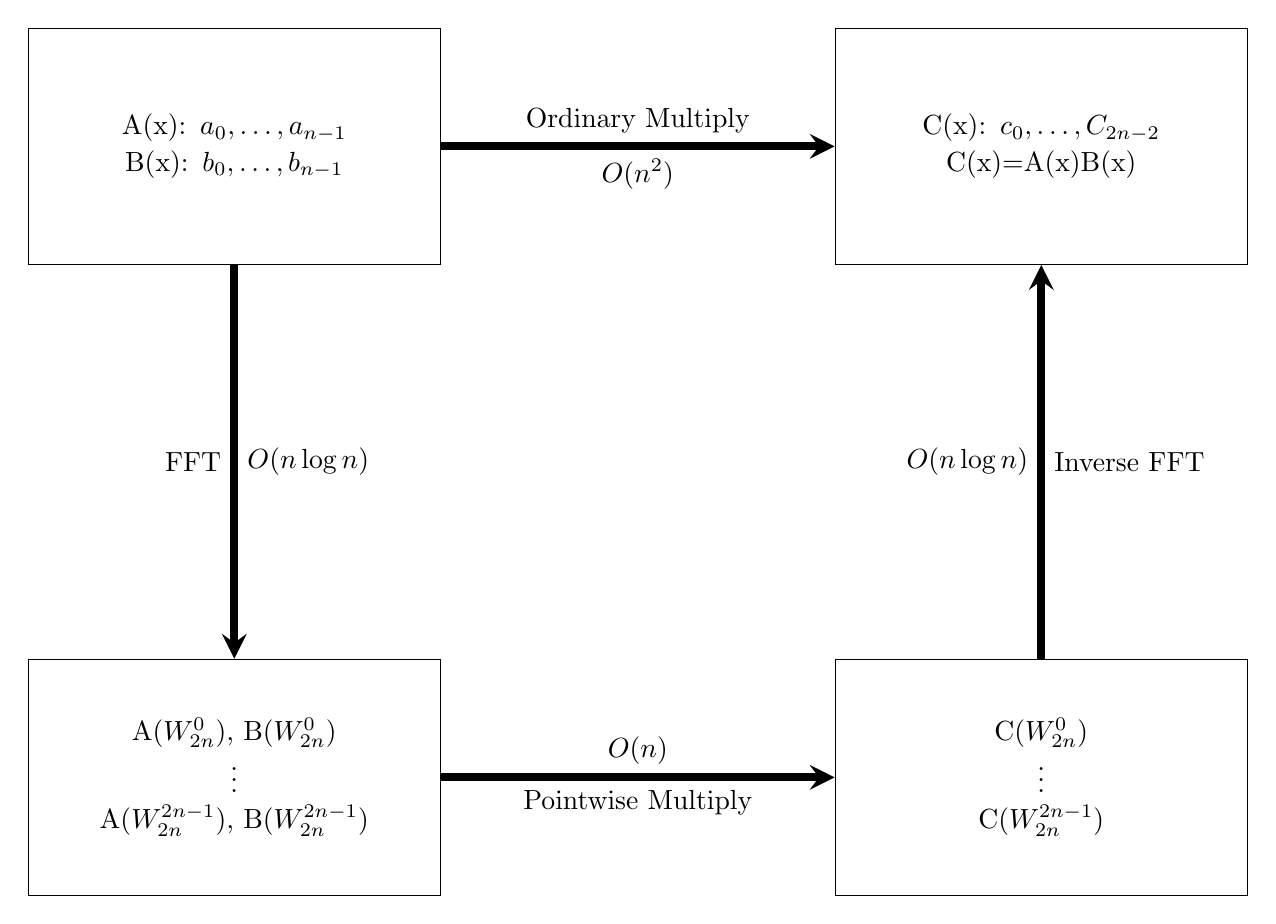
\begin{tikzpicture}[auto, node distance=5cm, box/.style={draw, rectangle, align=center, text width=5cm, minimum height=3cm, minimum width=5cm}, arrow/.style={draw, -stealth, line width=1mm}]
    % nodes
    \node[box] (A) {A(x): $a_0, \ldots, a_{n-1}$\\B(x): $b_0, \ldots, b_{n-1}$};
    \node[box] (B) [right=of A] {C(x): $c_0, \ldots, C_{2n-2}$\\C(x)=A(x)B(x)};
    \node[box] (C) [below=of A] {A($W_{2n}^0$), B($W_{2n}^0$)\\$\vdots$\\A($W_{2n}^{2n-1}$), B($W_{2n}^{2n-1}$)};
    \node[box] (D) [below=of B] {C($W_{2n}^{0}$)\\$\vdots$\\C($W_{2n}^{2n-1}$)};

    % arrows
    \draw[arrow] (A) -- node[above, draw=none] {Ordinary Multiply} node[below, draw=none] {$O(n^2)$} (B);
    \draw[arrow] (A) -- node[left, draw=none] {FFT} node[right, draw=none] {$O(n \log n)$} (C);
    \draw[arrow] (C) -- node[above, draw=none] {$O(n)$} node[below, draw=none] {Pointwise Multiply} (D);
    \draw[arrow] (D) -- node[left, draw=none] {$O(n \log n)$} node[right, draw=none] {Inverse FFT} (B);
\end{tikzpicture}

\textsf{In this problem, we take the coefficients of two polynomials A(x) and B(x) each with a degree of $n-1$ at the most, and we want to multiply them to get C(x). Instead of using ordinary multiplication which is $O(n^2)$, we can use the FFT polynomial multiplication algorithm to get a better efficiency.}

\subsection{Algorithm: Polynomial-Multiplication-FFT}
\noindent
\textbf{Input:} \\
$a = (a_0, ..., a_{n-1})$ \\
$b = (b_0, ..., b_{n-1})$

\vspace{10pt}

\noindent
\textbf{Output:} \\
$c = (c_0, ..., c_{2n-2})$

\vspace{10pt}

\noindent
\textbf{Algorithm Steps:}
\begin{enumerate}
    \item Run FFT(a, $\omega_{2n}$) and FFT(b, $\omega_{2n}$) to get $A(x)$ and $B(x)$ at the $(2n)^{th}$ roots of unity.
    \item Multiply to get $C(x) = A(x)B(x)$ at the $(2n)^{th}$ roots of unity.
    \item Run InverseFFT(C) to get $c = (c_0, ..., c_{2n-2})$.
\end{enumerate}

\vspace{10pt}

\subsection{Algorithm: FFT}
\noindent
\textbf{Input:} \\
$a = (a_0, ..., a_{n-1})$ \\
$\omega$, an $n^{th}$  root of unity

\vspace{10pt}

\noindent
\textbf{Output:} \\
$A(\omega^0),A(\omega^1),...,A(\omega^{n-1})$

\vspace{10pt}

\noindent
\textbf{Algorithm Steps:}
\begin{enumerate}
    \item if $\omega=1$, return $A(1)$
    \item Let $a_{even}=(a_0,a_2,...,a_{n-2})$ and $a_{odd}=(a_1,a_3,...,a_{n-1})$
    \item $(s_0,s_1,...,s_{\frac{n}{2}-1})=FFT(a_{even},\omega^2)$
    \item $(t_0,t_1,...,t_{\frac{n}{2}-1})=FFT(a_{odd},\omega^2)$
    \item For $j = 0 \xrightarrow{} \frac{n}{2} - 1$
    \begin{itemize}
        \item $r_j=s_j+\omega^jt_j$
        \item $r_{\frac{n}{2}+j}=s_j-\omega^jt_j$
    \end{itemize}
    \item Return $(r_0,r_1,...,r_{n-1})$
\end{enumerate}
\textsf{NOTE: in the above algorithm, $r_j$ represents $A(\omega^j)$, and $r_{\frac{n}{2}+j}$ represents $A(\omega^{j+\frac{n}{2}})$}

\section{Matrix View of FFT}
\textsf{For a polynomial A(x), when we apply $FFT(a,\omega_n)$, we get $A(\omega_n^0),A(\omega_n^1),...,A(\omega_n^{n-1})$. The following is a matrix representation of the FFT algorithm.}

\begin{enumerate}
    \item For points $x_0, x_1, ..., x_{n-1}$
\[
\begin{bmatrix}
    A(x_0) \\
    A(x_1) \\
    \vdots \\
    A(x_{n-1})
\end{bmatrix}
=
\begin{bmatrix}
    1 & x_0 & x_0^2 & \dots & x_0^{n-1} \\
    1 & x_1 & x_1^2 & \dots & x_1^{n-1} \\
    \vdots & \vdots & \vdots & \ddots & \vdots \\
    1 & x_{n-1} & x_{n-1}^2 & \dots & x_{n-1}^{n-1}
\end{bmatrix}
\begin{bmatrix}
    a_0 \\
    a_1 \\
    \vdots \\
    a_{n-1}
\end{bmatrix}
\]
    \item $x_j=\omega_n^j$ for $j=0,...,n-1$
\[
\begin{bmatrix}
    A(\omega_n^0) \\
    A(\omega_n^1) \\
    \vdots \\
    A(\omega_n^{n-1})
\end{bmatrix}
=
\textcolor{red}{
\begin{bmatrix}
    1 & 1 & 1 & \dots & 1 \\
    1 & \omega_n & \omega_n^2 & \dots & \omega_n^{n-1} \\
    \vdots & \vdots & \vdots & \ddots & \vdots \\
    1 & \omega_n^{n-1} & \omega_n^{2(n-1)} & \dots & \omega_n^{(n-1)(n-1)}
\end{bmatrix}}
\textcolor{blue}{
\begin{bmatrix}
    a_0 \\
    a_1 \\
    \vdots \\
    a_{n-1}
\end{bmatrix}}
\]
\begin{center}
$A=\textcolor{red}{M_n(\omega_n)}\textcolor{blue}{a}$
\end{center}
    \item Inverse FFT: $\textcolor{blue}{a}=\textcolor{red}{(M_n(\omega_n))^{-1}}A$

    \begin{center}
    \underline{Lemma} \\[10pt]
    $(M_n(\omega_n))^{-1}=\frac{1}{n}M_n(\omega_n^{-1})$ \\[10pt]
    $\omega_n=e^{\frac{2\pi{}i}{n}}$ \\
    $\omega_n^{-1}=\omega_n^{n-1}=e^{\frac{2\pi{}i}{n}(n-1)}$ \\[10pt]
    $m_n(\omega_n^{-1})=$
\[
\begin{bmatrix}
    1 & 1 & 1 & \dots & 1 \\
    1 & \omega_n^{-1} & \omega_n^{-2} & \dots & \omega_n^{-(n-1)} \\
    \vdots & \vdots & \vdots & \ddots & \vdots \\
    1 & \omega_n^{-(n-1)} & \omega_n^{-2(n-1)} & \dots & \omega_n^{-(n-1)(n-1)}
\end{bmatrix}
\]
\end{center}
\end{enumerate}

\section{Inverse FFT}
\noindent
Inverse FFT(C)\\
\textbf{Input:} \\
 \(C(\omega^0), C(\omega^1), ..., C(\omega^{2n-1})\) is a set of point-values \\

\vspace{10pt}

\noindent
\textbf{Output:} \\
\(c = (c_0, c_1, ..., c_{2n-1})\)\\

\vspace{10pt}

\noindent
\((S_0, S_1, ..., S_{2n-1}) = FFT(C, \omega_{2n}^{2n-1})\)\\
return \(\frac{1}{n}(S_0, S_1, ..., S_{2n-1})\) \(\rightarrow{}\) co-efficients of polynomial C(x)\\

\section{Example}


\[A(x) = 3 + x, B(x) = 2 + 2x\]
\noindent
Find C(x), where C(x) = A(x)B(x).\\
Based on the information of A(x) and B(X), we know that C(x) has degree of 2 (\(z^2\)) and will have 3 co-efficents. The power of 2 above 3 is 4 (\(2^2\)), so we will have 4 points of unity (\(\omega_4\)).\\
\vspace{10pt}

\noindent
Let \(a = (3,1)\), which is the co-efficients of degree 0 and 1 of A(x).\\
Let \(b = (2,2)\), which is the co-efficients of degree 0 and 1 of B(x).\\
\vspace{10pt}

\noindent
Now we run FFT with the inputs \((3,1)\) and \( \omega_4\).\\
\vspace{10pt}


We know that \(a_{even} = (3)\) which corresponds to the 0th degree of a. We also know that \(a_{odd} = (1)\) which corresponds to the 1st degree of a. Both of these correspond to \(\omega_2\).


\[FFT(a_{even}, \omega_{2}) = (3,3)\]
\[FFT(a_{odd}, \omega_{2}) = (1,1)\]
\noindent
The result of these (3,3) correspond to \((s_0,\)  \( s_1)\) and (1,1) correspond to \((t_0, t_1)\).\\
We can now calculate \((r_0, r_1, r_2,\) and \( r_3)\).\\
Additionally, \(\omega^{n}\) corresponds to \((1, i, -1,\) and \(-i)\) for n = 0,1,2, and 3 respectively.\\
\vspace{10pt}

\noindent
Remember that:
\begin{itemize}
        \item $r_j=s_j+\omega^jt_j$
        \item $r_{\frac{n}{2}+j}=s_j-\omega^jt_j$
    \end{itemize}
So for a(x),

\[r_0 = 3 + 1*1 = 4\]
\[r_1 = 3 + i*1 = 3 + i\]
\[r_2 = 3 - 1*1 = 2\]
\[r_3 = 3 - i*1 = 3-i\]
\noindent
thus, \(a(x) = (4, 3+i, 2, 3-i)\).\\
And for b(x),
\[r_0 = 2 + 1 = 4\]
\[r_1 = 2 + 2*i = 2 + 2i\]
\[r_2 = 2 + 2*(-1) = 0\]
\[r_3 = 2 + 2* (-i) = 2 - 2i\]
\noindent
thus,  \(b(x) = (4, 2+2i, 0, 2-2i)\).
We can now multiply the two together to get c(x), so \(r_0\) from a(x) * \(r_0\) from b(x) to get \(r_0\) for c(x).
\[r_0 = 4 * 4 = 16\]
\[r_1 = (3 + i)*(2+2i) = 4+8i\]
\[r_2 = 2 * 0 = 0\]
\[r_3 = (3 - i)*(2-2i) = 4-8i\]
This can now be run again on FFT, which looks like:

\[FFT((16,4+8i, 0, 4-8i), \omega_{4}^{3})\]









%FOR SCRIBES: ---------- End Scribing, begin biblio -----------------
%FOR SCRIBES: The first citation is just for telling you the style. Replace
%FOR SCRIBES: this with your citations if any. If there are no citations, just
%FOR SCRIBES: remove the bib environment.


%\bibliographystyle{plain}
%\begin{thebibliography}{10}
%\bibitem{mr:random}
%R.~Motwani and P.~Raghavan.
%\newblock {\em Randomized Algorithms}.
%\newblock Cambridge University Press, 1995.
%\end{thebibliography}

\end{document}
